\documentclass{article}

\usepackage[english]{babel}
\usepackage{svg}
\usepackage[letterpaper,top=2cm,bottom=2cm,left=3cm,right=3cm,marginparwidth=1.75cm]{geometry}

\usepackage{amsmath}
\usepackage{graphicx}
\usepackage[colorlinks=true, allcolors=blue]{hyperref}
\usepackage[autostyle, english = british]{csquotes}

\MakeOuterQuote{"}
\title{Local Complex-Action Gaussian Beam Propagation for Electron Microscope Forward Modelling}
\author{D. Landers}

\begin{document}
\maketitle

\begin{abstract}
Gaussian beam decomposition gives a compact way to propagate coherent wavefields through an optical system, because each beam carries a local centre, direction, phase, amplitude, and complex curvature. 
For electron microscope modelling this representation is attractive because lenses, apertures, biprisms, aberration functions, and projected sample transmission can all be described as local modifications to the optical action. 
Here we first revisit the propagation of shifted and tilted Gaussian beams through a common detector plane, where the terms usually described as misalignment phases are required to keep the amplitude and phase of each beam in the correct coordinates. 
We then use this observation to motivate a more general local complex-action update. 
Each thin component is represented by the value, gradient, and Hessian of a complex action around the Gaussian centre. 
The value updates the phase and amplitude, the gradient updates the beam direction and possible centre shift, and the Hessian updates the complex curvature. 
The method is exact for quadratic complex actions and approximate for higher-order structure over the support of each Gaussian beam.
\end{abstract}

\section{Introduction}

Forward models of electron microscopes must combine coherent wave propagation with a sequence of optical components. 
In a conventional grid-based calculation this is usually done by alternating transmission functions with free-space propagation. 
This representation is general, but it requires a sampled wavefield at every plane and can become expensive when many parameter changes or many optical elements must be evaluated.

Gaussian beam decomposition provides a complementary representation. 
The wavefield is written as a coherent sum of local Gaussian packets, and each packet can be propagated analytically through paraxial free space and through any component whose action is locally quadratic. 
The main difficulty is therefore not the propagation of one centred Gaussian, but the consistent bookkeeping of many shifted and tilted Gaussians in a shared detector plane. 
This point is already present in the Collins-integral treatment of misaligned optical systems, where terms that are linear in the input and output coordinates cannot in general be discarded when the final fields must be summed in a common plane.

The aim of this paper is to use that misalignment problem as the route into a more general method. 
Rather than deriving a separate closed form for every optical component, we describe each thin element by a local complex action. 
The real part represents phase or optical path length, while the imaginary part represents amplitude transmission. 
Taking the Taylor expansion of this complex action around each Gaussian beam gives the update rules for the beam centre, direction, amplitude, path length, and complex curvature. 
Apart from free-space propagation between planes, this is the calculation implemented in TemGymCore for Gaussian microscope forward modelling.

\section{The Collins Integral}

The 2D Collins integral, also known as the generalised Fresnel integral, enables the propagation of wavefields via $\mathbf{ABCD}$ transfer matrices:

\begin{align}
E_2\left(r_2\right) =& \frac{ik}{2\pi \sqrt{\det(\mathbf{B})}}
\exp\left(\frac{-ik}{2} \langle r_2|\mathbf{D}\mathbf{B}^{-1}|r_2\rangle\right) \notag \\
& \times \iint_{-\infty}^{\infty} E\left(r_1\right)
\exp\left(\frac{-ik}{2}\left[\langle r_1| \mathbf{B}^{-1} \mathbf{A}|r_1\rangle
- 2\langle r_1| \mathbf{B}^{-1}|r_2\rangle\right]\right) d^2 r_1
\label{eq:AlignedCollinsIntegral}
\end{align}

Here $r_1$ and $r_2$ are column vectors of coordinates $x$ and $y$ at the input and output planes, respectively. 
$\mathbf{A}$, $\mathbf{B}$, $\mathbf{C}$, and $\mathbf{D}$ are each diagonal $2 \times 2$ 
ray transfer matrices that permit astigmatic beam propagation. Here, $k$ is the wavenumber, and $E\left(r_1\right)$ is the input wavefield.   
The bra-ket notation conveniently encapsulates the vector-matrix dot product operation required to evaluate 
the terms of the Collins integral, where $\langle r |$ denotes $r^{T}$, the transpose of the column vector, and $|r\rangle$ 
denotes the same column vector without transpose, simply $r$. 
The calculation of a single column entry in, for example, $\langle r_1| \mathbf{B}^{-1}|r_2\rangle_j$ can be written as a 
summation, which more clearly demonstrates the operation:

\begin{equation}
\langle r_1 | \mathbf{B}^{-1} | r_2 \rangle_j = \sum_{i=1}^{2} \sum_{k=1}^{2} r_{1,i,j} \cdot \mathbf{B}^{-1}_{i,k} \cdot r_{2,k,j}
\label{eq:VectorMatrixProductSummation}
\end{equation}

where the subscript $j$ indicates that for each column element $j$ in $r_{1,i,j}$, 
the dot product matrix multiplication is performed. 
Note also that the normally present refractive index values $n_1$ and $n_2$ in Eq.~\eqref{eq:AlignedCollinsIntegral} are set to unity, 
resulting in a single wavenumber value $k = 2\pi/\lambda$, where $\lambda$ is the wavelength of the input wavefield.

\section{Gaussian Beams and Misaligned Optical Systems}

The utility of the Collins integral is that it gives an analytic propagation rule for Gaussian beams through a paraxial $\mathbf{ABCD}$ system. 
This is the starting point for Gaussian beam decomposition, where an arbitrary input wavefield is represented by a coherent sum of shifted and tilted Gaussian beams \cite{ashcraft_hybrid_2023, deschamps_gaussian_1971}. 
For an aligned Gaussian centred on the optical axis, the input field can be written as

\begin{equation}
E_1\left(r_1\right) = \exp\left(\frac{-ik}{2} \langle r_1 | \mathbf{Q}_{1}^{-1} | r_1 \rangle\right),
\label{eq:InputGaussianBeam}
\end{equation}

where $\mathbf{Q}_{1}^{-1}$ is the complex curvature matrix in the input plane. 
For an astigmatic but axis-aligned beam this is

\begin{equation}
\mathbf{Q}_1^{-1} = \begin{bmatrix}
q_{1xx}^{-1}(z) & 0 \\
0 & q_{1yy}^{-1}(z)
\end{bmatrix},
\label{eq:Q1_inv}
\end{equation}

with scalar entries

\begin{equation}
q_{1}^{-1}(z) = \frac{1}{R(z)} + i \frac{\lambda}{\pi w(z)^{2}} .
\label{eq:q1_inverse}
\end{equation}

Substitution into Eq.~\eqref{eq:AlignedCollinsIntegral} gives another Gaussian in the output plane,

\begin{equation}
E_2\left(r_2\right) = \exp\left(\frac{-ik}{2} \langle r_2 | \mathbf{Q}_{2}^{-1} | r_2 \rangle\right),
\label{eq:OutputGaussianBeam}
\end{equation}

where

\begin{equation}
\mathbf{Q}_{2}^{-1} = (\mathbf{C} + \mathbf{D} \mathbf{Q}_{1}^{-1})(\mathbf{A} + \mathbf{B} \mathbf{Q}_{1}^{-1})^{-1}.
\label{eq:Q2_invABCD}
\end{equation}

This aligned result is not enough for a beam-decomposition calculation. 
The input wavefield is represented by many Gaussian packets, and each packet has its own centre, tilt, amplitude, phase, and curvature. 
Once the packets are shifted and tilted, the problem is equivalent to a misaligned optical system. 
Previous treatments of misaligned systems often evaluate the field in a plane perpendicular to a centre-of-gravity ray \cite{weber_collins_2006, cai_propagation_2003}. 
For Gaussian beam decomposition in an electron microscope, however, all beams must be evaluated in the same detector plane so that they can be summed coherently.

\begin{figure}[h]
\centering
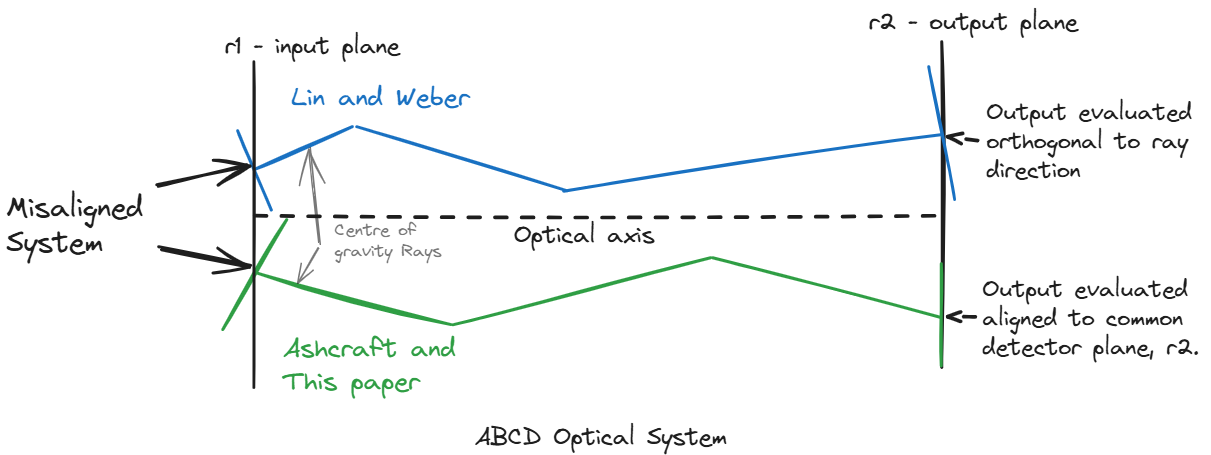
\includegraphics[width=0.8\textwidth]{MisalignedSystem.PNG}
\caption{Geometry of a shifted and tilted Gaussian beam propagated through a paraxial optical system. The detector-plane field must retain the phase and amplitude associated with the misaligned ray if many beams are to be summed coherently.}
\label{fig:MisalignedSystem}
\end{figure}

This distinction affects the algebra. 
Ashcraft et al.~\cite{ashcraft_generalized_2024} build on Weber's treatment and use an assumption that the linear terms vanish in the misaligned Collins integral. 
That cancellation is valid in the tilted output coordinate system used by Weber, but it does not generally hold when the output field is required in a common upright detector plane. 
The remaining linear terms are not a small correction to the aligned Gaussian. 
They encode the output centre, the local phase slope, and the phase origin of the propagated beam.

\section{Misaligned Gaussian Beam Solution}

We begin with a Gaussian displaced by $r_{1m}$ and tilted by $\theta_{1m}$ in the input plane:

\begin{equation}
E_1\left(r_1 - r_{1m}\right) = \exp\left(\frac{-ik}{2} \langle r_1 - r_{1m} | \mathbf{Q}_{1}^{-1} | r_1 - r_{1m} \rangle \right)
\exp\left(-ik \langle r_1 - r_{1m} | \theta_{1m} \rangle \right)
\label{eq:InputMisalignedGaussian}
\end{equation}

Here $r_{1m}$ and $\theta_{1m}$ are the input-plane centre and tilt of the beam. 
After the change of variables $r_1=\tilde{r}_1+r_{1m}$, the exponent contains only quadratic and linear terms in $\tilde{r}_1$. 
The Gaussian integral can therefore be evaluated analytically \cite{siegman_lasers_1986}. 
The important point is that the linear terms contain both the input displacement and the input tilt. 
Writing the propagated beam centre as

\begin{equation}
r_{2m} = \mathbf{A} r_{1m} + \mathbf{B} \theta_{1m},
\label{eq:MisalignedOutputCentre}
\end{equation}

the detector-plane field can be written compactly as

\begin{align}
E_2\left(r_2\right) = 
\Phi_{r_{1m}} \Phi_{r_{2m}} E_{2,\text{aligned}}\left(r_2\right)
\label{eq:MisalignedGaussianSolutionCondensed}
\end{align}

with

\begin{equation}
\begin{aligned}
E_{2,\text{aligned}}\left(r_2\right) &= 
\frac{1}{\sqrt{\det(\mathbf{A} + \mathbf{B} \mathbf{Q}_1^{-1})}}  
\exp\left(\frac{-ik}{2} \langle r_2 | \mathbf{Q}_2^{-1} | r_2 \rangle\right), \\
\Phi_{r_{1m}} &= \exp\left(\frac{-ik}{2} \left[ \langle r_{1m} | \mathbf{B}^{-1}\mathbf{A} | r_{1m} \rangle - 
2 \langle r_{1m} | \mathbf{B}^{-1} | r_2 \rangle \right] \right), \\
\Phi_{r_{2m}} &= \exp\left(\frac{-ik}{2} \left[ \langle r_{2m} | \mathbf{Q}_1 \mathbf{B}^{-1} (\mathbf{A}\mathbf{Q}_1 + \mathbf{B})^{-1} | r_{2m} \rangle 
- 2 \langle r_{2m} | \mathbf{Q}_1 \mathbf{B}^{-1} (\mathbf{A}\mathbf{Q}_1 + \mathbf{B})^{-1} | r_2 \rangle \right] \right)
\end{aligned}
\label{eq:MisalignedGaussianSolutionCondensedTerms}
\end{equation}

Equation~\eqref{eq:MisalignedGaussianSolutionCondensedTerms} contains the additional factor $\Phi_{r_{2m}}$ compared with the expression obtained when the linear terms are assumed to vanish. 
This factor moves the Gaussian envelope to the correct detector-plane centre and also moves the phase origin with it. 
In other words, the correction is not only an amplitude offset. 
It is the bookkeeping required to keep the centre, slope, phase, and curvature of each tilted Gaussian mutually consistent before coherent summation.

\section{Verification of the Misaligned Gaussian Beam Solution}

We verified Eq.~\eqref{eq:MisalignedGaussianSolutionCondensedTerms} against a direct Fresnel propagation calculation for a displaced Gaussian propagated through a thin lens. 
The test system follows the scale of the example in \cite{ashcraft_generalized_2024}: $\lambda = 1\,\mu\text{m}$, $w_0 = 3\,\text{mm}$, an input shift $x_0 = 5\,\text{mm}$, a focal length $f = 0.01\,\text{m}$, and an observation plane $z = 0.011\,\text{m}$ beyond the lens.

Figures~\ref{fig:CrossSection} and \ref{fig:2DImageMisalignedSystem} compare the corrected expression with the Fresnel reference. 
The detector-plane amplitude and phase are aligned only when the $\Phi_{r_{2m}}$ term is retained. 
An output-plane offset can move the amplitude envelope, but it does not by itself move the phase origin correctly. 
This is important in the cases considered below, where many Gaussian beams interfere after passing through aberrated elements or phase objects.

\begin{figure}[h]
\centering
\includegraphics[width=0.8\textwidth]{CrossSection.png}
\caption{Cross-section of the misaligned Gaussian beam propagation in the output plane.}
\label{fig:CrossSection}
\end{figure}

\begin{figure}[h]
\centering
\includegraphics[width=0.8\textwidth]{2DImageMisalignedSystem.png}
\caption{2D image of the misaligned optical system in the output plane.}
\label{fig:2DImageMisalignedSystem}
\end{figure}

\section{Local Complex-Action Gaussian Beam Propagation}

The corrected misaligned solution suggests a more general viewpoint. 
Rather than deriving a new Collins-integral expression for every tilted, shifted, absorbing, or aberrated element, we store each Gaussian beam as a local action expansion in a common plane. 
In this section $Q_j$ denotes the inverse complex-curvature matrix stored with beam $j$, using the sign convention of the implementation. 
A positive imaginary part of $Q_j$ gives a decaying Gaussian envelope because the field is written as

\begin{equation}
E_j(r)=a_j\exp\left(ik\left[S_j+\theta_j^T\delta r+\frac{1}{2}\delta r^TQ_j\delta r\right]\right),
\quad \delta r=r-r_j .
\label{eq:GaussianStateLocalAction}
\end{equation}

Here $r_j$ is the beam centre, $\theta_j$ is the local propagation angle, $S_j$ is the accumulated path-length action at the centre, and $a_j$ is the complex amplitude. 
This representation keeps exactly the quantities that the misalignment calculation showed must remain consistent: centre, slope, phase, amplitude, and curvature.

A thin optical component is represented by a complex action increment

\begin{equation}
\Delta \mathcal{S}(r)=\Delta S(r)-\frac{i}{k}\log T(r),
\label{eq:ComplexActionDefinition}
\end{equation}

where $\Delta S(r)$ is the phase or path-length contribution and $T(r)$ is an amplitude transmission. 
This form is useful because the physical transmission factor is recovered by $\exp(ik\Delta\mathcal{S})$. 
If $0<T<1$, then $\log T<0$ and the imaginary part of $\Delta\mathcal{S}$ attenuates the Gaussian amplitude by the factor $\exp[-k\,\operatorname{Im}(\Delta\mathcal{S})]$.

For each beam, the component is sampled locally by Taylor expanding Eq.~\eqref{eq:ComplexActionDefinition} around the beam centre:

\begin{equation}
\Delta\mathcal{S}(r_j+\delta r)\approx
\Delta\mathcal{S}_0+\Delta\mathcal{S}_1^T\delta r+\frac{1}{2}\delta r^T\Delta\mathcal{S}_2\delta r .
\label{eq:ComplexActionTaylor}
\end{equation}

If the component action is exactly quadratic over the beam support, this update is exact. 
For higher-order aberrations, sharp apertures, or samples, the neglected terms are the cubic and higher residuals over the finite width of the beam. 
The direct local update is

\begin{equation}
\tilde{S}_j=S_j+\Delta\mathcal{S}_0,\quad
\tilde{\theta}_j=\theta_j+\Delta\mathcal{S}_1,\quad
\tilde{Q}_j=Q_j+\Delta\mathcal{S}_2 .
\label{eq:DirectComplexActionUpdate}
\end{equation}

When the transmission varies across the Gaussian, $\tilde{\theta}_j$ can be complex. 
The imaginary part shifts the maximum of the Gaussian envelope away from the previous centre. 
The recentering step used here is

\begin{equation}
\Delta r_c = -(\operatorname{Im}\tilde{Q}_j)^{-1}\operatorname{Im}\tilde{\theta}_j .
\label{eq:ComplexRecentering}
\end{equation}

After this shift, the beam state is written again about the new envelope maximum:

\begin{equation}
\begin{aligned}
r'_j &= r_j+\Delta r_c, \\
S'_j &= \operatorname{Re}\left[\tilde{S}_j+\tilde{\theta}_j^T\Delta r_c+\frac{1}{2}\Delta r_c^T\tilde{Q}_j\Delta r_c\right], \\
a'_j &= a_j\exp\left(-k\,\operatorname{Im}\left[\tilde{S}_j+\tilde{\theta}_j^T\Delta r_c+\frac{1}{2}\Delta r_c^T\tilde{Q}_j\Delta r_c\right]\right), \\
\theta'_j &= \operatorname{Re}\left(\tilde{\theta}_j+\tilde{Q}_j\Delta r_c\right), \\
Q'_j &= \tilde{Q}_j .
\end{aligned}
\label{eq:RecentredGaussianState}
\end{equation}

In the absence of amplitude gradients, Eq.~\eqref{eq:ComplexRecentering} gives no centre shift and the update reduces to the usual phase-gradient and phase-curvature update. 
With an absorbing aperture or sample transmission, the same equations also describe attenuation, a small shift toward higher transmission, and a change in beam width from the curvature of $\log T$.

Between thin components the beam is propagated exactly in paraxial free space. 
For a distance $L$,

\begin{equation}
\begin{aligned}
r'_j &= r_j+L\theta_j, \\
S'_j &= S_j+L+\frac{1}{2}L\,\theta_j^T\theta_j, \\
Q'_j &= Q_j(I+LQ_j)^{-1}, \\
a'_j &= a_j\det(I+LQ_j)^{-1/2}.
\end{aligned}
\label{eq:FreeSpaceGaussianUpdate}
\end{equation}

Apart from this free-space step, all thin elements use the same local coefficient extraction. 
The change between a lens, an aperture, a biprism, and a sample is therefore not the Gaussian update itself, but the scalar function from which $\Delta\mathcal{S}_0$, $\Delta\mathcal{S}_1$, and $\Delta\mathcal{S}_2$ are obtained.

\section{Component Examples}

A thin lens or stigmator is a quadratic phase element. 
For a centred lens, $\Delta S(r)=-(x^2+y^2)/(2f)$, with separate focal lengths in $x$ and $y$ for a stigmator. 
Since this action is quadratic, Eq.~\eqref{eq:ComplexActionTaylor} is exact and the Hessian update gives the usual curvature change.

Aberrated lenses use the same update, but the phase is no longer purely quadratic. 
For example, Krivanek or Seidel aberration functions add higher-order terms to the ideal lens action. 
The local update keeps the value, gradient, and Hessian at each Gaussian centre, so it captures the local deflection and curvature of the aberrated wavefront. 
The approximation that remains is the cubic and higher residual across the beam support.

A soft aperture is naturally described by $\log T(r)$ rather than only by a binary mask. 
The value of $\log T$ attenuates the beam, its gradient shifts the beam centre toward higher transmission, and its Hessian changes the Gaussian width near an absorbing edge. 
This is a local approximation to the aperture transmission, and its accuracy depends on the aperture edge being resolved by the Gaussian packet width or by additional beam splitting.

A biprism can also be treated as a component action. 
Away from the wire the phase is locally close to a ramp, so the first derivative gives the angular deflection. 
Near the wire, the absolute-value phase and finite transmission width introduce non-quadratic structure, but the coefficient extraction remains the same as for the lens and aperture.

Projected sample transmission fits the same complex-action framework, but it is not made the main claim of the present theory section. 
For atomic potentials, the local Taylor expansion at an atom core can be a poor model even when the action is smooth, because the curvature can vary rapidly over the beam support. 
In those cases a sampled fitted quadratic over the Gaussian support may be more appropriate than a derivative Taylor expansion at the centre.

\section{Forward Microscope Model}

The forward model is a single pass through an ordered microscope model. 
First, the input wave is decomposed into a bundle of Gaussian beams. 
Each beam is propagated in free space to the next component using Eq.~\eqref{eq:FreeSpaceGaussianUpdate}. 
The component then supplies a phase shift and, where needed, a log-transmission, which are converted into the local complex-action coefficients in Eq.~\eqref{eq:ComplexActionTaylor}. 
The beam state is updated and recentred using Eqs.~\eqref{eq:DirectComplexActionUpdate}--\eqref{eq:RecentredGaussianState}. 
After all components have been applied, the detector field is evaluated by summing Eq.~\eqref{eq:GaussianStateLocalAction} over the final Gaussian bundle.

In TemGymCore this corresponds to a small set of operations. 
Components provide \texttt{phase\_shift} and optionally \texttt{log\_transmission}. 
\texttt{FreeSpacePropagator} applies the paraxial propagation step, \texttt{apply\_action\_delta} applies the local complex-action update and recentres the beam, and the detector evaluation coherently sums the resulting Gaussian fields. 
This implementation detail is not essential to the derivation, but it makes the method straightforward to extend because a new thin component only needs to define its local action.

\section{Validation Strategy}

The current validation should be read as a set of targeted checks rather than a complete benchmark suite. 
The misaligned-lens case checks the detector-plane phase bookkeeping against Fresnel propagation. 
The aperture examples check the effect of log-transmission against a direct Fresnel calculation through the same mask. 
The biprism examples test coherent interference from beams that acquire different local phase ramps. 
The aberrated-aperture examples compare Taylor Gaussian propagation with Fresnel and angular-spectrum references for a fixed Krivanek phase plate. 
Finally, the higher-order residual diagnostics measure when the local quadratic approximation is no longer sufficient and when fitted quadratics or beam splitting are needed.

\bibliographystyle{unsrt}
\bibliography{references}

\end{document}
